\documentclass[a4paper]{scrartcl}
\usepackage{amsmath,amssymb,amsthm}
\usepackage{bm}
\usepackage{biblatex}
\usepackage{caption}
\usepackage{float}
\usepackage[colorlinks=true, allcolors=black, urlcolor=cyan]{hyperref}
\usepackage{graphicx}
\usepackage[framed,numbered]{matlab-prettifier}
\usepackage{mathtools}
\usepackage{mcode}
\usepackage{physics}
\usepackage{siunitx}
\usepackage{cancel}
\usepackage{appendix}

\renewcommand{\thesection}{\Roman{section}}
\renewcommand{\thesubsection}{\roman{subsection})}

\title{Assignment 4}
\subtitle{ELEC 442 - Introduction to Robotics}
\author{Sondre Myrberg (81113433) \and Ola Helbaek (68776772)}


\setlength{\parindent}{0pt} % Disable indentation
\mathtoolsset{showonlyrefs} % Only show equation numbers on referenced equations

\def\undertilde#1{\mathord{\vtop{\ialign{##\crcr
$\hfil\displaystyle{#1}\hfil$\crcr\noalign{\kern1.5pt\nointerlineskip}
$\hfil\widetilde{}\hfil$\crcr\noalign{\kern1.5pt}}}}} %Lousy way, but need this undertilde
\newcommand{\me}[1]{\mathrm{e}^{#1}}


\begin{document}

\hypersetup{pageanchor=false}
\begin{titlepage}
    \maketitle
    \vfill
    \vfill
    \vfill
    \vfill
    
\includegraphics[width=0.95\textwidth]{../../ubc_logo.pdf}
    \vfill
    \vfill
\end{titlepage}
\hypersetup{pageanchor=true}

\section{Two-Link Manipulator Open Loop Simulation}
Considering the two link manipulator described on page 87 in chapter 6 of the notes, the equations of motion are given by equation (209) to (233). In general we have the Euler-Lagrange equations of motion given as
\begin{equation}
	\begin{aligned}
		\dv{t}\left[\pdv{L}{\dot{q}_i} (q,\dot{q}) \right] - \pdv{L}{q_i} (q,\dot{q}) &= \tau_i \\
	\end{aligned}
\end{equation}
where
\begin{equation}
	\begin{aligned}
		L(\bm{q},\dot{\bm{q}}) &= T(\bm{q},\dot{\bm{q}}) - V(\bm{q})
	\end{aligned}
\end{equation}
and $\tau_i$ is the generalized force or torque associated with coordinate $i$. This can be written on standard form as
\begin{equation}
	\begin{aligned}
		D(\bm{q})\ddot{\bm{q}} + C(\bm{q},\dot{\bm{q}})\dot{\bm{q}} + G(\bm{q}) &= \bm{u} + \underline{J}^\top_n \begin{bmatrix} \underline{f}_e \\ \underline{\tau}_e \end{bmatrix}
	\end{aligned}
\end{equation} 
where the last term can be ignored as we do not interact with the environment. This gives us the secod order system
\begin{equation}
	\begin{aligned}
		\ddot{\bm{q}} &= D^{-1}(\bm{q})\left[\bm{u} - C(\bm{q},\dot{\bm{q}})\dot{\bm{q}} - G(\bm{q}) \right]
	\end{aligned}
\end{equation}
with $D(\bm{q})$ given by equation (222), $C(\bm{q},\dot{\bm{q}})$ given by (232) and $G(\bm{q})$ by (233), and $\bm{q} = \begin{bmatrix}
	\theta_1 \\ \theta_2
\end{bmatrix}$. To generate these matrices in Simulink, we implement block functions shown in \autoref{fig:genC}, \autoref{fig:genD} and \autoref{fig:genG} in \autoref{sec:simulink}. The complete mainpulator dynamics are implemented in \autoref{fig:dynamics}.

\subsection{}
With $\bm{x}(0) = \begin{bmatrix}0 & 0 & 0 & 0\end{bmatrix}^\top$ and $\tau_1 = \tau_2 = 0$ we get the response shown in \autoref{fig:1i_1}.

\begin{figure}[ht!]
	\centering
	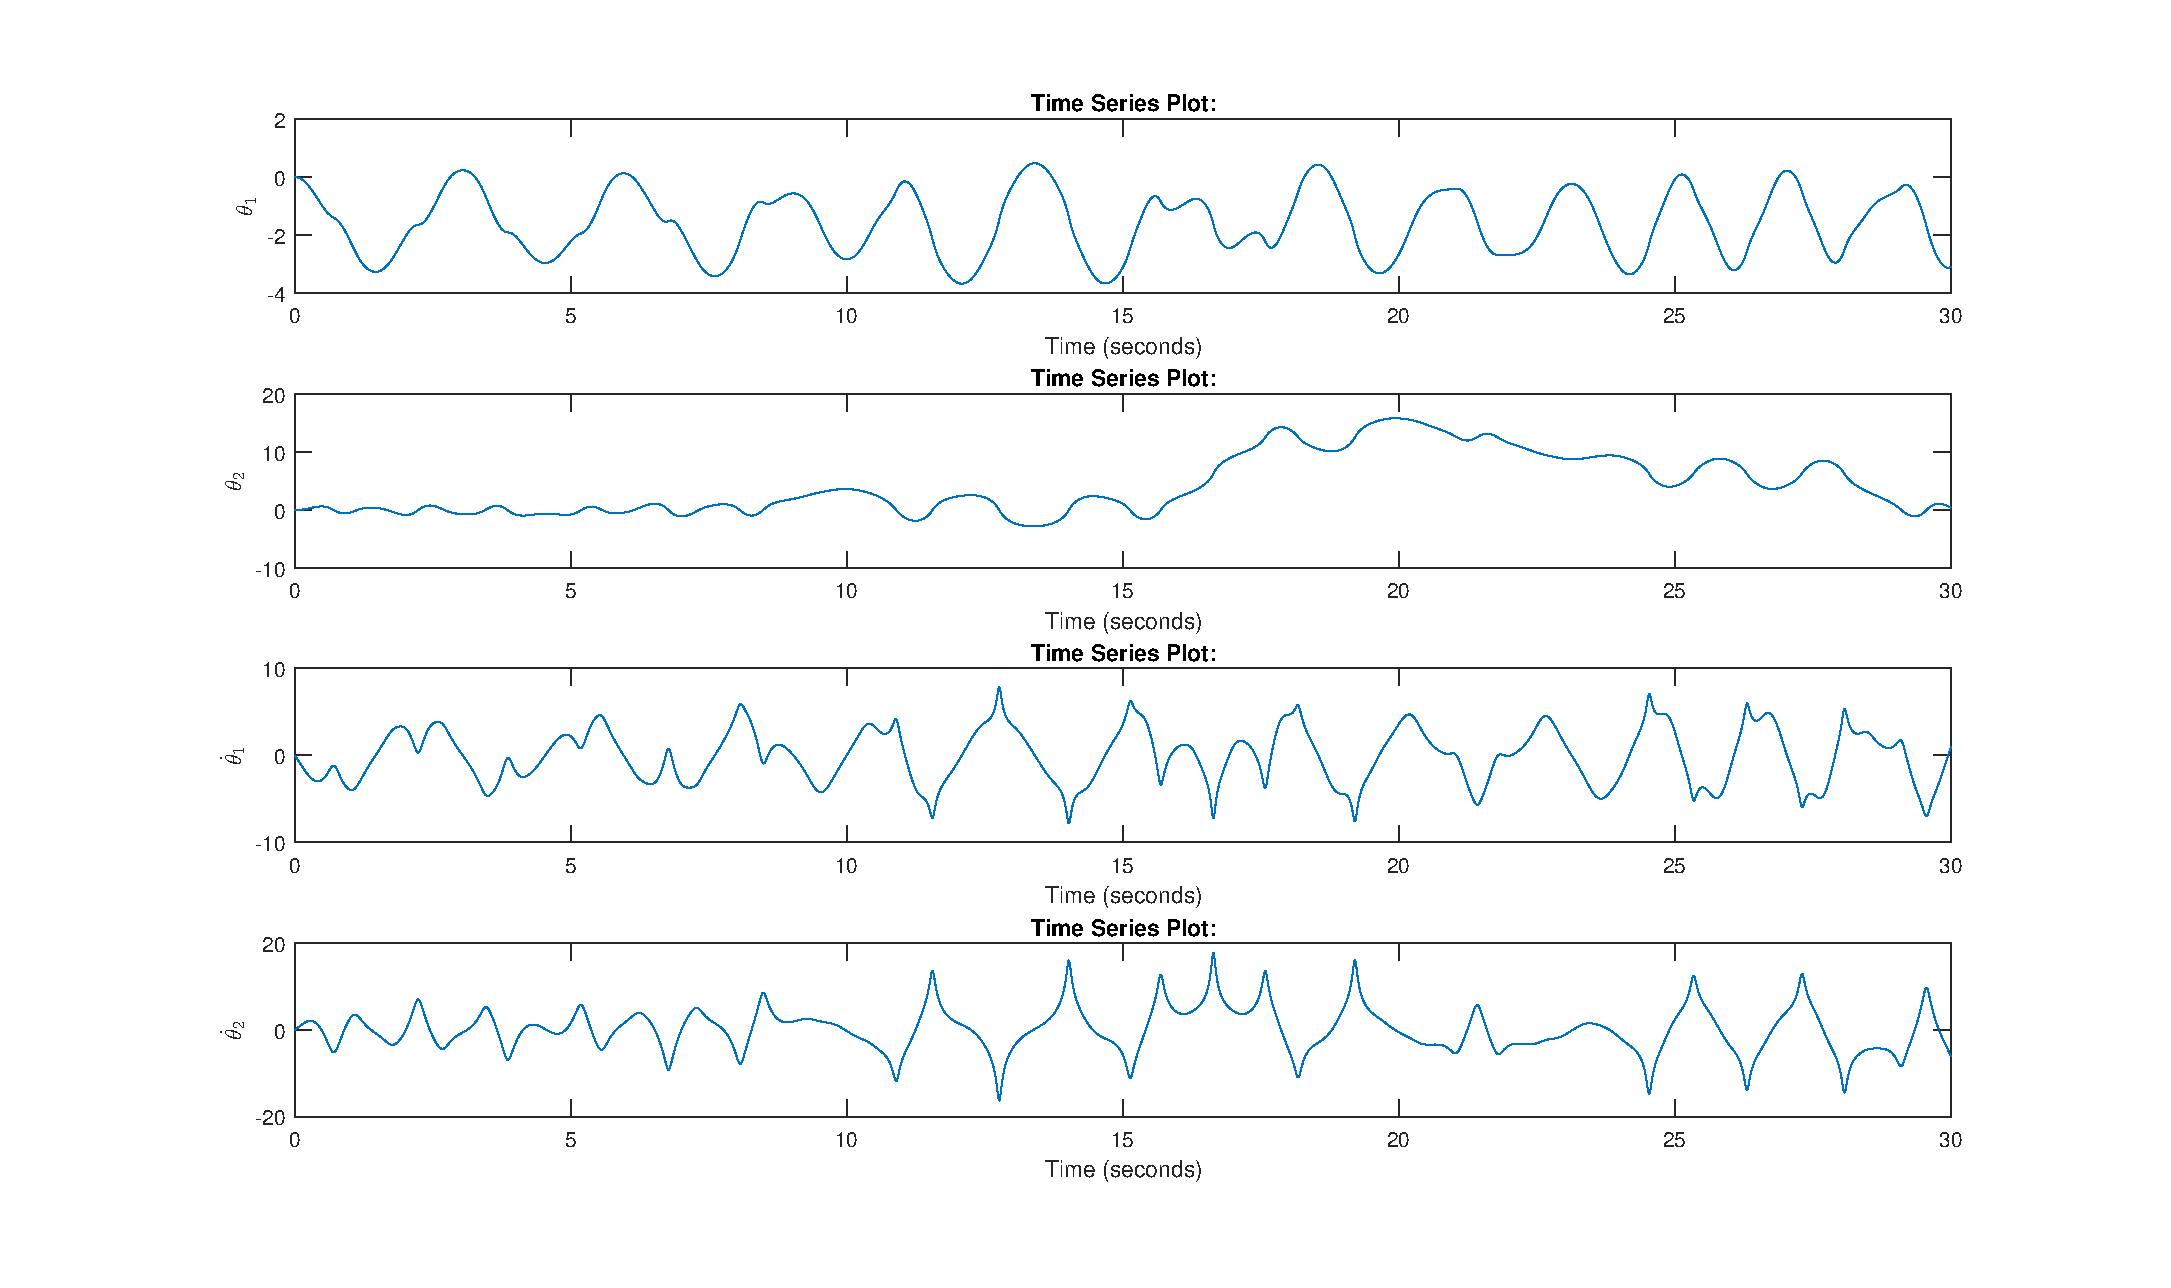
\includegraphics[width=.90\textwidth]{fig/1i_1.eps}
	\caption{Response of all states with all states initialized to zero}
	\label{fig:1i_1}
\end{figure}

\subsection{}
With $\bm{x}(0) = \begin{bmatrix}0 & \tfrac{\pi}{2} & 0 & 0\end{bmatrix}^\top$ and $\tau_2 = \SI{5}{Nm}$ we get the response shown in \autoref{fig:1ii_1}. Here the total energy of the system is increasing, which is seen in the plots for the angular velocities.

\begin{figure}[ht!]
	\centering
	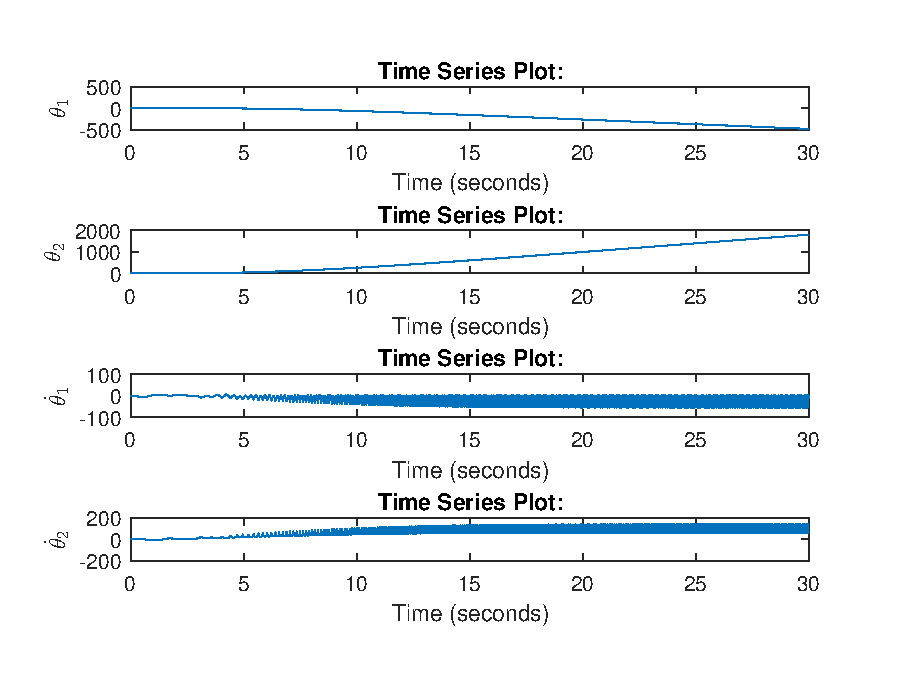
\includegraphics[width=.90\textwidth]{fig/1ii_1.eps}
	\caption{Response of all states with  $\bm{x}(0) = \left[0 \: \tfrac{\pi}{2} \: 0 \: 0\right]^\top$ and $\tau_2 = \SI{5}{Nm}$}
	\label{fig:1ii_1}
\end{figure}

\subsection{}
With $\bm{x}(0) = \begin{bmatrix}0 & 0 & 0 & 0\end{bmatrix}^\top$ and friction modeled as $\tau_1 = -0.5\dot{\theta}_1$ and $\tau_2 = -0.5\dot{\theta}_2$ we get the response shown in \autoref{fig:1iii_1}. Here we see that the amplitude is decreasing, wich makes sense because the total energy of the system is decreasing when friction is added.

\begin{figure}[ht!]
	\centering
	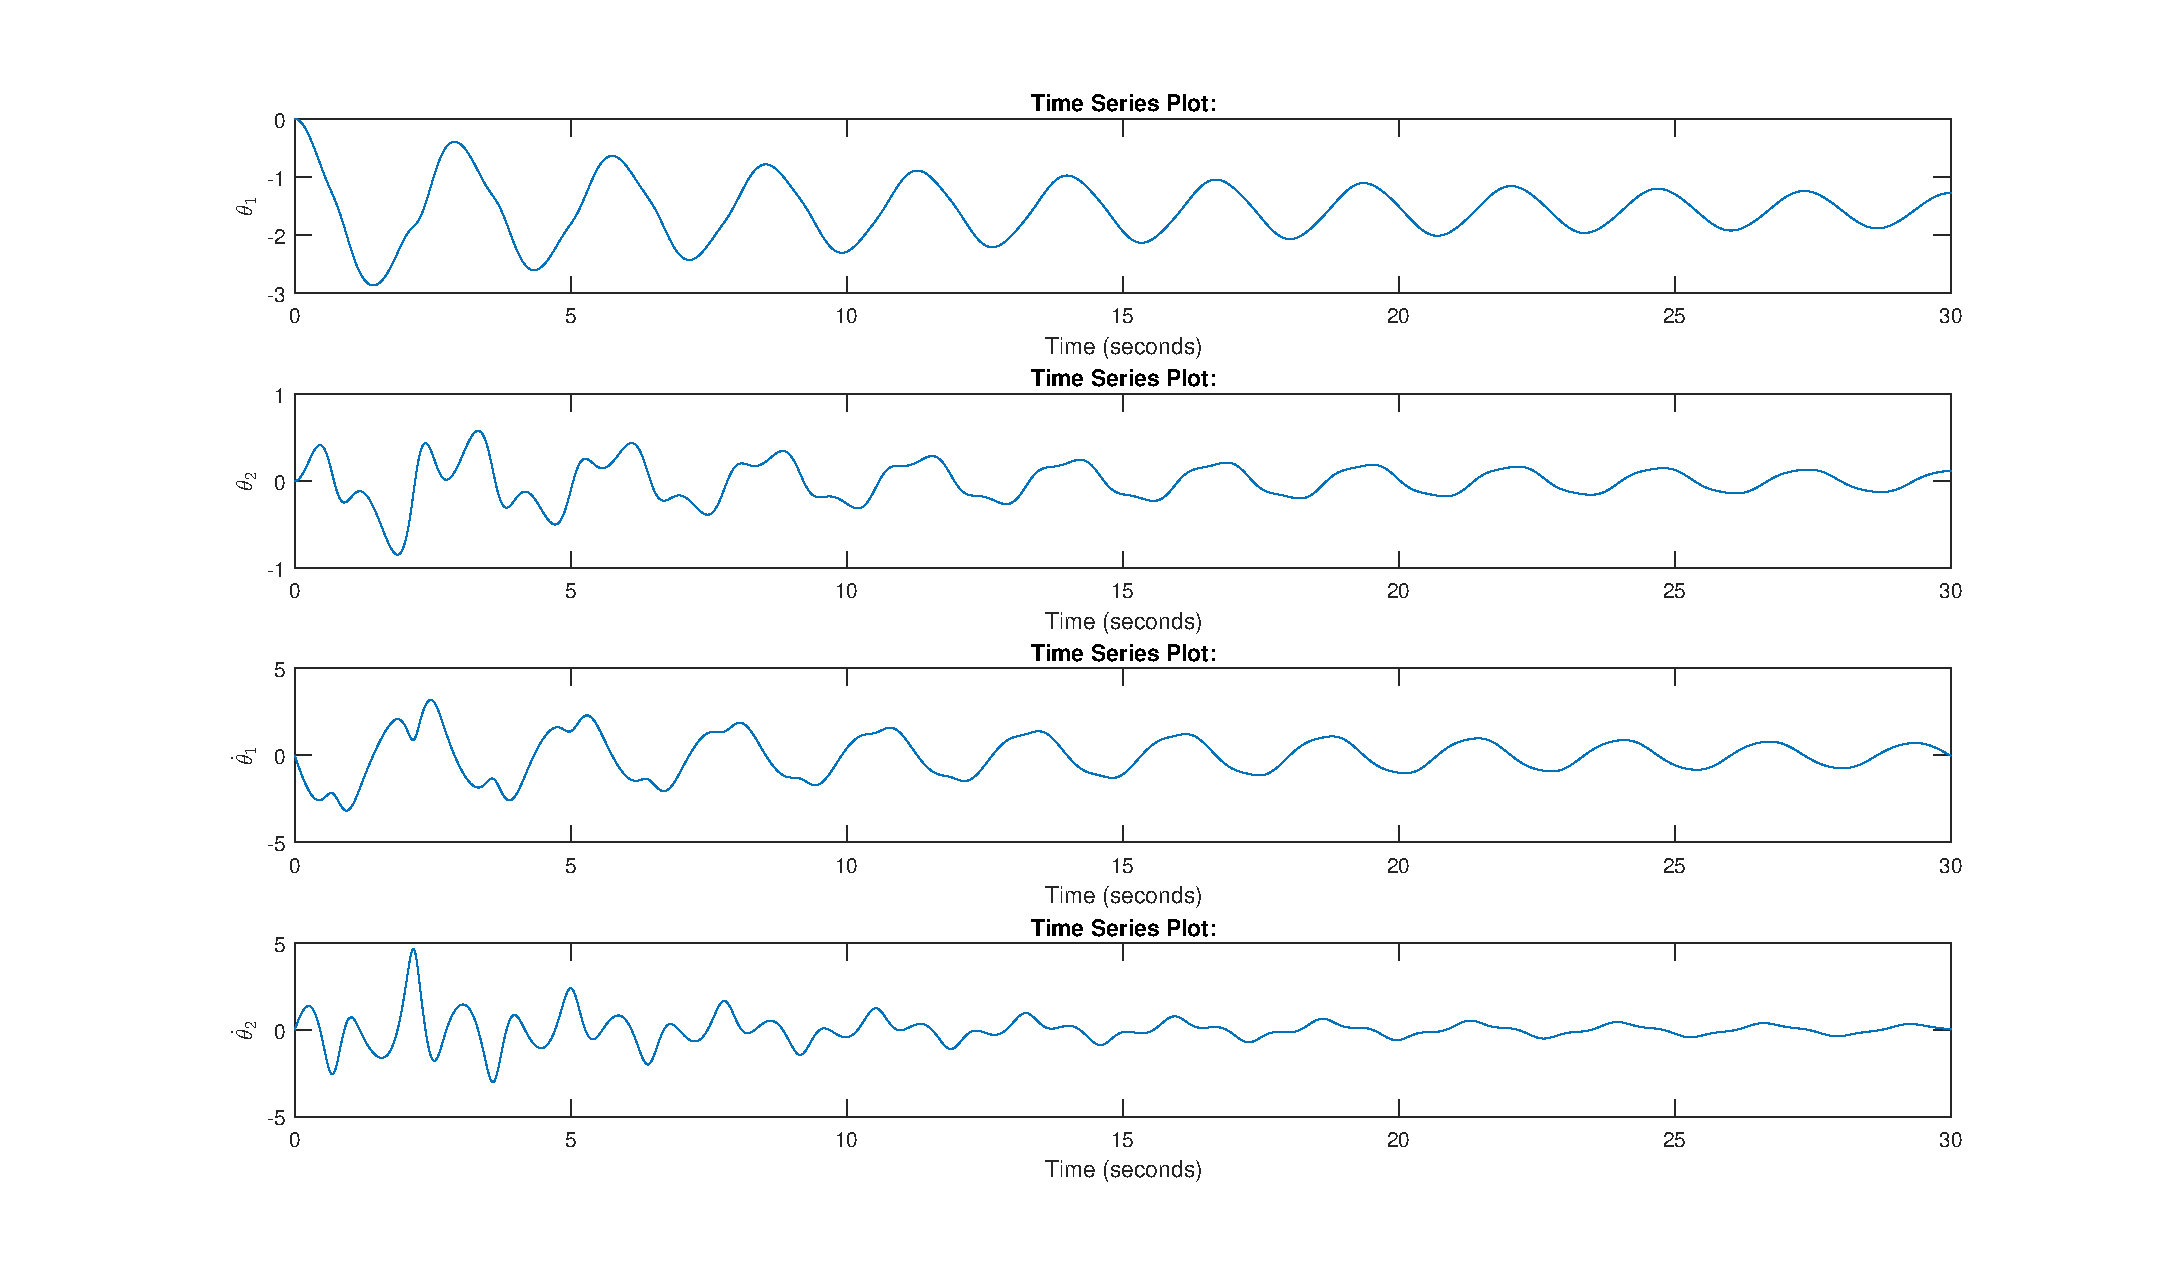
\includegraphics[width=.90\textwidth]{fig/1iii_1.eps}
	\caption{Response of all states with  all states initialized to zero and friction modeled as  $\tau_1 = -0.5\dot{\theta}_1$ and $\tau_2 = -0.5\dot{\theta}_2$ }
	\label{fig:1iii_1}
\end{figure}

\section{Controller Implementation}
\subsection{Closed loop joint-space control}
With the PD + gravity controller we get the input vector
\begin{equation}
	\begin{aligned}
		\bm{u} &= \underbrace{G(\bm{q})}_{\text{Gravity terms}} + \underbrace{K_p(\bm{q}_d - \bm{q}) - K_v \dot{\bm{q}}}_{\text{PD-controller}}
	\end{aligned}
\end{equation}
where we require
\begin{equation}
	K_p, K_v \succ 0
\end{equation}
which is implemented as the Simulink diagram shown in \autoref{fig:PDgravity}. With this implementation and the initial conditions 
\begin{equation}
	\begin{aligned}
		\bm{x}(0) &= \begin{bmatrix} -\tfrac{\pi}{2} & 0 & 0 & 0 \end{bmatrix}^\top \\
		\bm{q}_d &= \begin{bmatrix} 0 & \tfrac{\pi}{2} \end{bmatrix}^\top \\
		K_p &= \begin{bmatrix} 1 & 0 \\ 0 & 1 \end{bmatrix}\\
		K_v &= \begin{bmatrix} 2 & 0 \\ 0 & 2 \end{bmatrix}\\
	\end{aligned}
\end{equation}
we get the output shown in \autoref{fig:2PD_1}.

\begin{figure}[ht]
	\centering
	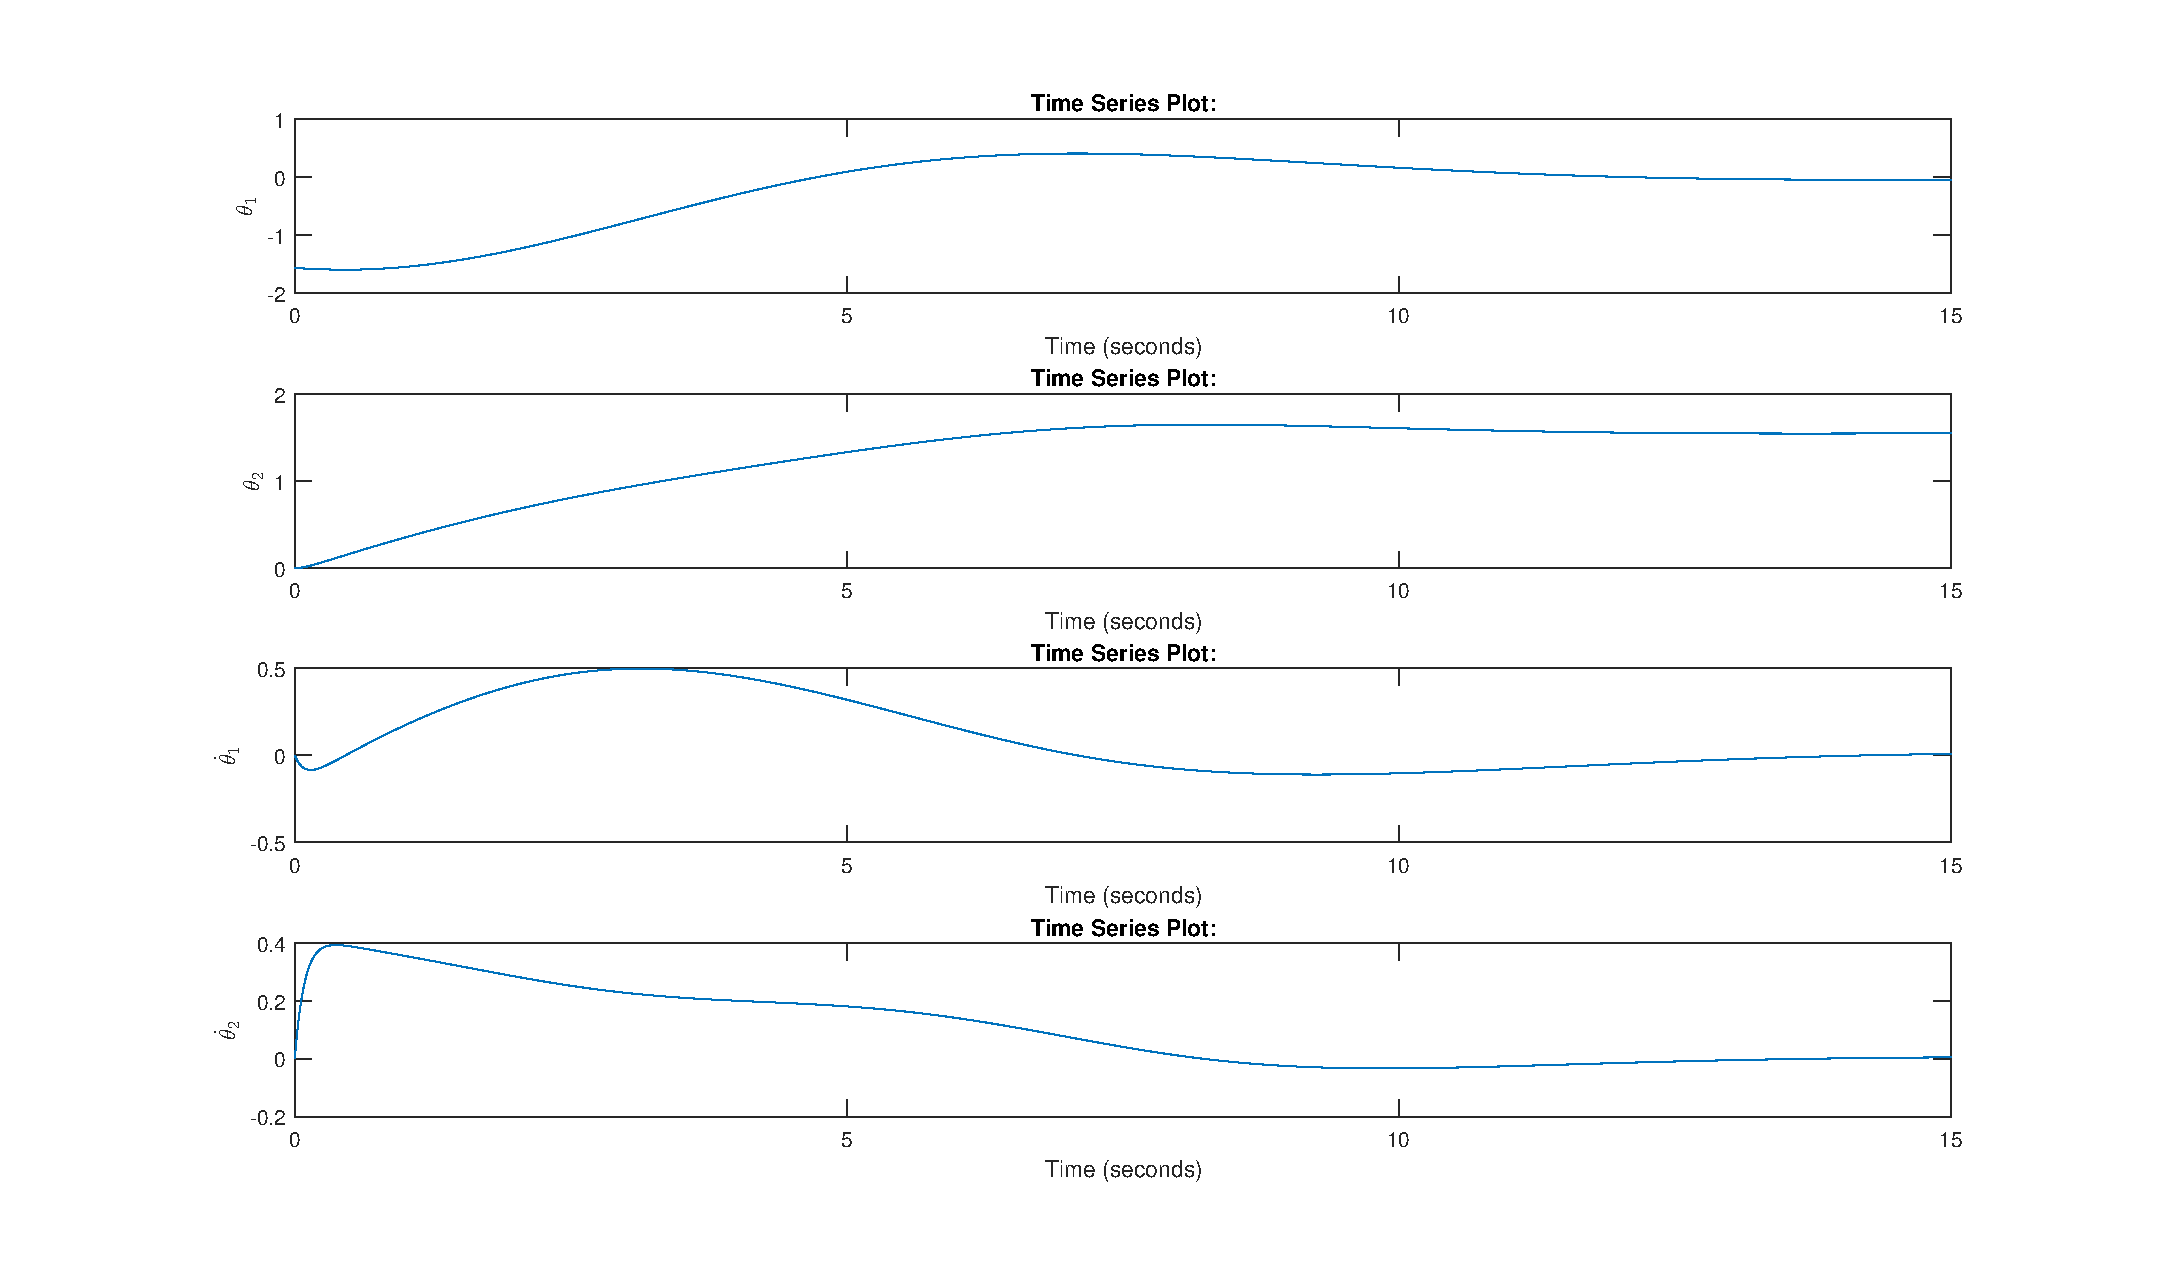
\includegraphics[width=0.95\textwidth]{fig/2PDg_1.eps}
	\caption{Output states with the PD + gravity controller}
	\label{fig:2PD_1}
\end{figure}

\clearpage
\appendix
\appendixpage
\addappheadtotoc
\section{Simulink diagrams}\label{sec:simulink}
\begin{figure}[ht]
	\centering
	\includegraphics[width=0.70\textwidth]{fig/C_func.pdf}
	\caption{Simulink function block to generate $C(\bm{q}, \dot{\bm{q}})$}
	\label{fig:genC}
\end{figure}
\begin{figure}[ht]
	\centering
	\includegraphics[width=0.75\textwidth]{fig/D_func.pdf}
	\caption{Simulink function block to generate $D(\bm{q})$}
	\label{fig:genD}
\end{figure}
\begin{figure}[ht]
	\centering
	\includegraphics[width=0.75\textwidth]{fig/G_func.pdf}
	\caption{Simulink function block to generate $G(\bm{q})$}
	\label{fig:genG}
\end{figure}
\begin{figure}[ht]
	\centering
	\includegraphics[width=0.95\textwidth]{fig/dynamics.pdf}
	\caption{Simulink block to the complete manipulator dynamics}
	\label{fig:dynamics}
\end{figure}
\begin{figure}[ht]
	\centering
	\includegraphics[width=0.95\textwidth]{fig/PDgravity.pdf}
	\caption{Simulink block for the PD + gravity controller}
	\label{fig:PDgravity}
\end{figure}



\end{document}